\section{Sampling}\label{dist-samp}
In the Machine Learning and Optimization literature, SGD algorithms are optimized to avoid scanning the entire data.
Uniform sampling is cheap so it is the preferred solution.
However, there are a few observations about the data cleaning problem that suggest that we can do better if we carefuly select which points to clean.
The key property that we need to preserve is unbiasedness of the gradient (Proposition \ref{unbiased}), so our updates are on average correct.

\vspace{0.5em}

\noindent\textbf{Use the partitioning: }
We first select a set of records before starting we select a set of dirty records $R_{dirty} \subseteq R$. 
We construct batch $S_{dirty}$ only from the dirty records and apply cleaning to this batch.
Now the problem is that this sample (and the resulting gradient) is possibly biased since we are excluding some data.
However, since we know that the set $R_{clean} = R - R_{dirty}$ is clean, we can compute the average gradient over those records without cleaning:
\[
g_C(\theta^{t}) = \frac{1}{\mid R - R_{dirty} \mid} \sum g_i(\theta^{t})
\]
Since we know the partition sizes, we can combine the two estimates $g_C$ and $g_S$ togther:
\[
g(\theta^{t}) = \frac{\mid R_{dirty} \mid \cdot g_S + \mid R_{clean} \mid \cdot g_C  }{\mid R \mid}
\]
Therefore,
\[
\alpha = \frac{R_{clean}}{R}, \beta = \frac{R_{dirty}}{R} \blacksquare
\]

\begin{lemma}
The gradient estimate $g(\theta^{t})$ is unbiased if $g_S$ is an unbiased estimate of:
\[
\frac{1}{\mid R_{dirty} \mid} \sum g_i(\theta^{t})
\]
\end{lemma}
\begin{proof}[Sketch]
This result follows directly from the linearity of expectation, since we are adding a deterministic result with an unbiased result.
\end{proof}

\vspace{0.5em}

\noindent\textbf{Optimal Sampling Problem: }
In this problem, we are trying to select a sample $S_{dirty}$ from $R_{dirty}$.
If we sample every element $i \in R_{dirty}$ with probability $p_i$, the question is
how can we compute a set of $\{p_i\}$ such that variance of the gradient $\sigma^2$ is minimized.  
It will turn out that optimal distribution is not realizable without knowing the fully cleaned data, and we will address this problem in the next section.
To construct these sampling probabilities, we first need the following lemma:
\begin{lemma}\label{impsample}
Given a set of real numbers $A = \{a_1,...,a_n\}$, let $\hat{A}$ be 
a sample with replacement of $A$ of size k.
If $\mu$ is the mean $\hat{A}$, the sampling distribution that minimizes
 the variance of $\mu$, i.e., the expected square error, is $p(a_i) \propto a_i$.
\end{lemma}
\begin{proof}[Sketch]
This proof follows from \cite{mcbook}, as it is a straight forward importance sampling result.
It is easy to verify that for sampling probabilities $p(a_i)$, that the unbiased
estimate of the mean is:
\[
\mu = \frac{1}{nk}\cdot\sum_{i\in\hat{A}}^k \frac{a_i}{p_i}
\]
If we minimize the variance $Var(\mu)$, we can find that:
\[
p_i = \frac{\mid a_i \mid }{\sum_i \mid a_i \mid}
\]
\end{proof}

\iffalse
The variance of this estimate is given by:
\[
Var(\mu) = \mathbb{E}(\mu^2)-\mathbb{E}(\mu)^2
\] 
Since the estimate is unbiased, we can replace $\mathbb{E}(\mu)$ with the average of $A$:
\[
Var(\mu) = \mathbb{E}(\mu^2)-\bar{A}^2
\]
Since $\bar{A}$ is deterministic, we can remove that term during minimization.
Furthermore, we can write $\mathbb{E}(\mu^2)$ as:
\[
\mathbb{E}(\mu^2) = \frac{1}{n^2}\sum_i^n \frac{a_i^2}{p_i}
\]
Then, we can solve the following optimization problem (removing the proportionality of $\frac{1}{n^2}$) over the set of weights $P=\{p(a_i)\}$:
\[
\min_{P} \sum_i^N \frac{a_i^2}{p_i}
\]
\[
\text{subject to: } P > 0, \sum P = 1
\]
Applying Lagrange multipliers, an equivalent unconstrained optimization problem is:
\[
\min_{P > 0,\lambda > 0} \sum_i^N \frac{a_i^2}{p_i} + \lambda \cdot (\sum P - 1)
\]
If, we take the derivatives with respect to $p_i$ and set them equal to zero:
\[
-\frac{a_i^2}{2 \cdot p_i^2} + \lambda = 0
\]
If, we take the derivative with respect to $\lambda$ and set it equal to zero:
\[
\sum P - 1
\]
Solving the system of equations, we get:
\[
p_i = \frac{\mid a_i \mid }{\sum_i \mid a_i \mid}
\]
\fi


Based on Lemma \ref{impsample}, we now derive an optimal sampling distribution.
Lemma \ref{impsample} shows that when estimating a mean of numbers with sampling, the distribution with optimal variance is where we sample proportions to the values.
We visualize this intuition in Figure \ref{update-arch3}, and essentially, this lemma shows
that when estimating a function of a random variable $\mathbb{E}(f(X))$ the optimal sampling distribution is to align the samples as closely as possible with the function.
This is insight leads to a direct higher-dimensional generalization, where at iteration $t$ we should sample the records in $R_{dirty}$ with probabilities:
\[
p_i \propto \|\nabla\phi(x^{(clean)}_i,y^{(clean)}_i,\theta^t)\|
\]
This is an insight which has recently been of great interest in the Machine Learning community \cite{zhao2014stochastic}.
However, in our case, it leads to a chicken-and-egg problem.
The optimal sampling distribution requires knowing $(x^{(clean)}_i,y^{(clean)}_i)$, however, we have to sample and clean those points to get $(x^{(clean)}_i,y^{(clean)}_i)$.
In the next section, we discuss how to inexpensively approximate this optimal distribution.
As our technique can work with \emph{any} distribution, we are guaranteed convergence no matter how inaccurate this approximation.
However, a better approximation will lead to an improved convergence rate.

\begin{figure}[ht!]
\centering
 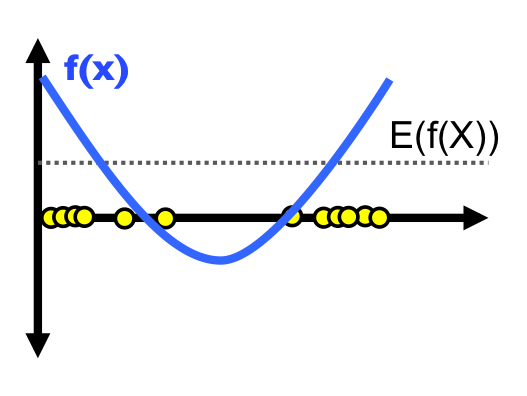
\includegraphics[width=0.6\columnwidth]{figs/update-arch3.png}
 \caption{The minimum variance estimate of an expected value of a function of a random variable $\mathbb{E}(f(X))$ is found by placing more samples (marked in yellow) on the higher parts of the function.\label{update-arch3}}
\end{figure}